\documentclass[a4paper,12pt]{article}
\usepackage{Template/_preamble}


%%--- TITLE PAGE text variables
%% replace with your information

\renewcommand{\title}{Thesis Title} % title is forced to uppercase
\renewcommand{\author}{Author One } % if more than one author, use below and comment this out
% \renewcommand{\author}{Author One \\ Author Two} % place a linebreak after every author
\renewcommand{\date}{May 2023} % Month Year

\renewcommand{\department}{Electronics Engineering Department} % edit the whole line
\renewcommand{\college}{College of Engineering and Architecture} % edit the whole line
\renewcommand{\degree}{Bachelor of Science in Electronics Engineering} % edit the whole line



%%--- ABSTRACT
%% write your abstract here
\renewcommand{\abstract}{
Lorem ipsum dolor sit amet, consectetur adipiscing elit, sed do eiusmod tempor incididunt ut labore et dolore magna aliqua. Ut enim ad minim veniam, quis nostrud exercitation ullamco laboris nisi ut aliquip ex ea commodo consequat. Duis aute irure dolor in reprehenderit in voluptate velit esse cillum dolore eu fugiat nulla pariatur. Excepteur sint occaecat cupidatat non proident, sunt in culpa qui officia deserunt mollit anim id est laborum.

Lorem ipsum dolor sit amet, consectetur adipiscing elit, sed do eiusmod tempor incididunt ut labore et dolore magna aliqua. Ut enim ad minim veniam, quis nostrud exercitation ullamco laboris nisi ut aliquip ex ea commodo consequat. Duis aute irure dolor in reprehenderit in voluptate velit esse cillum dolore eu fugiat nulla pariatur. Excepteur sint occaecat cupidatat non proident, sunt in culpa qui officia deserunt mollit anim id est laborum.

Lorem ipsum dolor sit amet, consectetur adipiscing elit, sed do eiusmod tempor incididunt ut labore et dolore magna aliqua. Ut enim ad minim veniam, quis nostrud exercitation ullamco laboris nisi ut aliquip ex ea commodo consequat. Duis aute irure dolor in reprehenderit in voluptate velit esse cillum dolore eu fugiat nulla pariatur. Excepteur sint occaecat cupidatat non proident, sunt in culpa qui officia deserunt mollit anim id est laborum.
}
%% write your keywords here (provde 3-5 indexing phrases that collectively describe the study)
\renewcommand{\keywords}{Keyword 1, Keyword 2, Keyword 3, Keyword 4, Keyword 5}



%%--- ACKNOWLEDGMENT
%% write your acknowledgment here
\renewcommand{\acknowledgment}{
Lorem ipsum dolor sit amet, consectetur adipiscing elit, sed do eiusmod tempor incididunt ut labore et dolore magna aliqua. 

Ut enim ad minim veniam, quis nostrud exercitation ullamco laboris nisi ut aliquip ex ea commodo consequat. Duis aute irure dolor in reprehenderit in voluptate velit esse cillum dolore eu fugiat nulla pariatur. Excepteur sint occaecat cupidatat non proident, sunt in culpa qui officia deserunt mollit anim id est laborum.
}





%%--- START OF MAIN PAPER
\begin{document}

%%--- show the title page
\pagenumbering{roman}
\addtocontents{toc}{\string\contentsline{section}{\normalfont \protect\hyperlink{titlepage}{TITLE PAGE}}{\normalfont\thepage} \\}

\begin{titlepage}
    \begin{center}
    
        \hypertarget{titlepage}{}
        {\bfseries\large\MakeUppercase \title }
        
        \vspace{1\baselineskip}

        \begin{figure}[h]
            \centering
            
\includegraphics[height=5.5cm]{Template/USTP-logo.png}
        \end{figure}

        \vspace{1\baselineskip}

        An \\
        Undergraduate Thesis \\
        Presented to the Faculty of \\
        \department \\
        \college \\

        \vspace{1\baselineskip}
        
        In Partial Fulfillment of the Requirements for the Degree of \\
        \degree \\

        \vspace{2\baselineskip}

        {\bfseries \author }

        \vspace{3\baselineskip}

        { \date }
 

    \end{center}
\end{titlepage}

\setcounter{page}{2} % start counting from (ii), because title page is (i)


%%--- comment out unused pages
\addtocontents{toc}{\string\contentsline{section}{\normalfont \protect\hyperlink{approvalsheet}{APPROVAL SHEET}}{\normalfont\thepage} \\}

\begin{center}

    {\bfseries \hypertarget{approvalsheet}{APPROVAL SHEET} }

    \vspace{1\baselineskip}

    \textcolor{red}{\textit{(see FM-USTP-ACAD-11 Approval Sheet)}}

\end{center}

\clearpage{}
\addtocontents{toc}{\string\contentsline{section}{\normalfont ABSTRACT}{\normalfont\thepage} \\}

\begin{center}

    {\bfseries ABSTRACT }
    \vspace{1\baselineskip}

\end{center}

    \abstract

    \vspace{1\baselineskip}
    \noindent Keywords: \textit{\keywords}

\clearpage{}
\addtocontents{toc}{\string\contentsline{section}{\normalfont \protect\hyperlink{acknowledgment}{ACKNOWLEDGMENT}}{\normalfont\thepage} \\}

\begin{center}

    {\bfseries \hypertarget{acknowledgment}{ACKNOWLEDGMENT} }
    \vspace{1\baselineskip}

\end{center}

    \acknowledgment

\clearpage{}
\addtocontents{toc}{\string\contentsline{section}{\normalfont \protect\hyperlink{tableofcontents}{TABLE OF CONTENTS}}{\normalfont\thepage} \\}

%% Only in Table of Contents we compress the line spacing to 1.5
{
\onehalfspacing
    \hypertarget{tableofcontents}{}
    \tableofcontents{}
\doublespacing
}

\clearpage{}
\addtocontents{toc}{\string\contentsline{section}{\normalfont \protect\hyperlink{listoffigures}{LIST OF FIGURES}}{\normalfont\thepage} \\}
\hypertarget{listoffigures}{}
\listoffigures{}	
\clearpage{}
\addtocontents{toc}{\string\contentsline{section}{\normalfont \protect\hyperlink{listoftables}{LIST OF TABLES}}{\normalfont\thepage} \\}
\hypertarget{listoftables}{}
\listoftables{}	
\clearpage{}

%%--- reset the page counting
\pagenumbering{arabic}
\setcounter{page}{1}


%%--- revise as needed
\section{INTRODUCTION}
\label{sec:INTRODUCTION}

%=======================
%--- Subsection 1.1 ---%
\subsection{Background of the Study}

Read \cref{sec:INTRODUCTION} for learning the basics of how to write in LaTeX and \cref{sec:REVIEW OF RELATED LITERATURE} for learning how to do citations. Moreover, glance \cref{sec:METHODOLOGY} and \cref{sec:RESULTS AND DISCUSSION} for manipulating figures and tables respectively.

Unless you know what you are doing, do not touch the Template folder, especially the preamble file as these files define the formatting. Replace the information for title page, abstract, keywords, and acknowledgment in main tex file with your own. Revise the Chapters, Tables, and Images folders as needed. Add your references data in the references.bib file.


%=======================
%--- Subsection 1.2 ---%
\subsection{Statement of the Problem}

\noindent Lists are easy to create:
\begin{itemize}
  \item List entries start with the \verb|\item| command.
  \item Individual entries are indicated with a black dot, a so-called bullet.
  \item The text in the entries may be of any length.
\end{itemize}


%=======================
%--- Subsection 1.3 ---%
\subsection{Objectives of the Study}

\noindent Numbered (ordered) lists are easy to create:
\begin{enumerate}
  \item Items are numbered automatically.
  \item The numbers start at 1 with each use of the \texttt{enumerate} environment.
  \item Another entry in the list
\end{enumerate}


%=======================
%--- Subsection 1.4 ---%
\subsection{Conceptual Framework}

    \begin{figure}[ht]
        \caption{Conceptual Framework of Camera-Based System With Voice Feedback}
        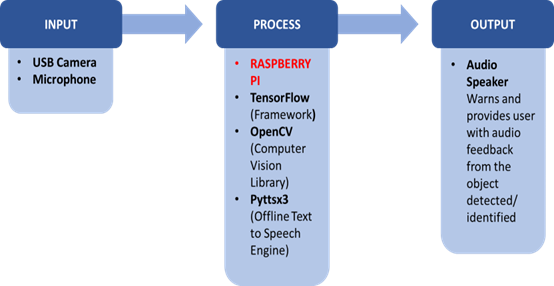
\includegraphics[width=1\textwidth]{Images/conceptual-framework.png}
        \label{fig:concept-frame}
    \end{figure}

You can put more than one value in the parameter, for instance, if you write [ht] LATEX will try to position the figure here, but if it's not possible (the space may be insufficient) then the figure will appear at the top of the page (See \autoref{table:pos-params} for more parameters). It is recommended to use more than one positioning parameter to prevent unexpected results.

To reference the figure, just call the label of the figure using \verb|\autoref|, i.e. \autoref{fig:concept-frame}, and it will automatically generate the correct reference. Resize the figure by changing this parameter \verb|[width=1\textwidth]| (this default means stretch the figure to occupy the whole width of the paper).


%=======================
%--- Subsection 1.5 ---%
\subsection{Significance of the Study}

    % insert the table for positioning parameters for Figures and Tables in LATEX
    \definecolor{ShuttleGray}{rgb}{0.364,0.407,0.474}
\begin{table}[ht]
\centering
\caption{Figure and Tables positioning parameters}
\begin{tblr}{
  width = \linewidth,
  colspec = {Q[69]Q[867]},
  cells = {fg=ShuttleGray},
  hline{2-8} = {-}{},
}
\textbf{Param} & \textbf{Position}                                                                                                                                                                                                                                                                                      \\
h              & \textcolor[rgb]{0.365,0.408,0.475}{Place the float~\textit{here\textcolor[rgb]{0.365,0.408,0.475}{, i.e.,~\textit{approximately\textcolor[rgb]{0.365,0.408,0.475}{~at the same point it occurs in the source text (however, not~\textit{exactly\textcolor[rgb]{0.365,0.408,0.475}{~at the spot)}}}}}}} \\
t              & \textcolor[rgb]{0.365,0.408,0.475}{Position at the~\textit{top\textcolor[rgb]{0.365,0.408,0.475}{~of the page.}}}                                                                                                                                                                                      \\
b              & \textcolor[rgb]{0.365,0.408,0.475}{Position at the~\textit{bottom\textcolor[rgb]{0.365,0.408,0.475}{~of the page.}}}                                                                                                                                                                                   \\
p              & \textcolor[rgb]{0.365,0.408,0.475}{Put on a special~\textit{page\textcolor[rgb]{0.365,0.408,0.475}{~for floats only.}}}                                                                                                                                                                                \\
!              & Override internal parameters LaTeX uses for determining "good" float positions.                                                                                                                                                                                                                        \\
H              & Places the float at precisely the location in the~LATEX~code. Requires the~float~package. This is somewhat equivalent to~h!.                                                                                                                                                                           
\end{tblr}
\label{table:pos-params}
\end{table}

Referencing tables is similar to referencing figures mentioned earlier, \autoref{table:pos-params}. To create hyperlinks, use \verb|\href| or \verb|\url|. For example, you can learn more about tables in this \href{https://www.overleaf.com/learn/latex/Tables}{link} or easily generate tables in LATEX format in this url: \url{https://www.latex-tables.com/}


%=======================
%--- Subsection 1.6 ---%
\subsection{Scope and Limitations}

Formulas should be used if they support the explanation. For formulas, LaTeX is ideal.
A formula should - if it is not extremely short - be presented in a separate line. For referencing, formulas should be numbered consecutively with Arabic numbers. The numbers should be aligned right in the last line of a formula. Formulas and variables must always be explained in the text.

Example: The following formula describes the expected mean snake length LQ of a (M/M/1) system, where represents the expected utilization:
\begin{equation}
       LQ=  \frac{\rho^2}{1-\rho} 
\end{equation}


%=======================
%--- Subsection 1.7 ---%
\subsection{Definition of Terms}

\noindent Change the labels using \verb|\item[label text]| in a \texttt{description} environment
\begin{description}
     \item[Note:] I would like to describe something here
     \item[Caveat!] And give a warning here
     \item[Term 1.] Lorem ipsum dolor sit amet, consectetur adipiscing elit, sed do eiusmod tempor incididunt ut labore et dolore magna aliqua.
     \item[Term 2.] Lorem ipsum dolor sit amet, consectetur adipiscing elit, sed do eiusmod tempor incididunt ut labore et dolore magna aliqua.
\end{description}
\section{REVIEW OF RELATED LITERATURE}
\label{sec:REVIEW OF RELATED LITERATURE}

The reference section is auto-generated based on your references.bib, and are sorted alphabetically. There are two ways to cite in-text, namely:

\subsection{Citing with parencite}

\verb|\parencite{reference label}| is used for in-text citation outside the sentence structure. You can label your references in many ways, but I recommend using the AuthorYear (i.e. Rotman2009) naming convention for a cleaner implementation \parencite{Rotman2009}. This is how it will look when citing two authors \parencite{booktwoauthors} and three authors \parencite{bookthreeauthors} from a book using \verb|@book|.

To cite from a journal paper, use \verb|@article| \parencite{journalarticleoneauthor}. You can also place multiple labels in one citation call just like this \parencite{journalarticletwoauthors, journalarticlethreeauthors}. To cite a conference paper or book chapter, use \verb|@incollection| \parencite{bookchapter} and to cite a website use \verb|@misc| \parencite{website}.


\subsection{Citing with textcite}

\verb|\textcite{reference label}| is used for in-text citation within the sentence structure. You can label your references in many ways, but I recommend using the AuthorYear (i.e. Rotman2009) naming convention for a cleaner system, as shown in \textcite{Rotman2009}. This is how it will look when citing two authors \textcite{booktwoauthors} and three authors \textcite{bookthreeauthors} from a book using \verb|@book|.

To cite from a journal paper, use \verb|@article| exemplified in \textcite{journalarticleoneauthor}. You can also place multiple labels in one citation call just like \textcite{journalarticletwoauthors, journalarticlethreeauthors}. To cite a conference paper or book chapter, use \verb|@incollection| from \textcite{bookchapter}. Furthermore, to cite a website use \verb|@misc| illustrated in \textcite{website}.
\section{METHODOLOGY}
\label{sec:METHODOLOGY}

\subsection{Manipulating Figures}

\autoref{fig:flow-chart} is an example of adjusting the figure to only 50\% of the page width and formatting it in center-alignment.

    \begin{figure}[ht]
        \caption{System Flow Chart of Object Recognition with Voice Feedback}
        \centering
        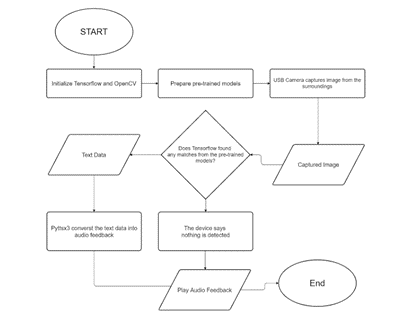
\includegraphics[width=0.5\textwidth]{Images/system-flow-chart.png}
        \label{fig:flow-chart}
    \end{figure}

\subsection{Manipulating Figures}

Meanwhile \autoref{fig:power-circuit} is an example of adjusting the figure to 80\% of the page width and formatting it right-aligned using \verb|\raggedleft|.

    \begin{figure}[ht]
        \caption{Power Supply Circuit}
        \raggedleft
        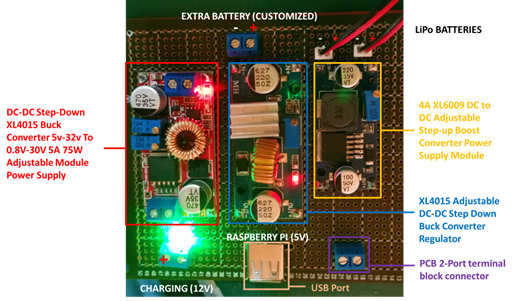
\includegraphics[width=0.8\textwidth]{Images/power-supply-circuit.png}
        \label{fig:power-circuit}
    \end{figure}
\section{RESULTS AND DISCUSSION}
\label{sec:RESULTS AND DISCUSSION}

\subsection{Simple Table}

\noindent \autoref{table:simple} shows how to create a simple table, but you can also easily generate tables with LaTeX using this url: \url{https://www.latex-tables.com/}

\verb|\hline| will insert a horizontal line on top of the table and at the bottom too. There is no restriction on the number of times you can use \verb|\hline|. Each \& is a cell separator and the double-backslash \verb|\\|  sets the end of this row.

    \begin{table}[htbp]
    \caption{Creating a Simple Table}
    \begin{center}
    \begin{tabular}{ |c|c|c| } 
     \hline
     cell1 & cell2 & cell3 \\ 
     cell4 & cell5 & cell6 \\ 
     cell7 & cell8 & cell9 \\ 
     \hline
    \end{tabular}
    \end{center}
    \label{table:simple}
    \end{table}


\subsection{Combining rows and columns}

\noindent \autoref{table:multirow} shows how to combine rows by using the multirow package:

    \begin{table}[htbp]
    \caption{Table with multiple rows and columns}
    \begin{tabular}{ |p{3cm}||p{3cm}|p{3cm}|p{3cm}|  }
     \hline
     \multicolumn{4}{|c|}{Country List} \\
     \hline
     Country Name or Area Name& ISO ALPHA 2 Code &ISO ALPHA 3 Code&ISO numeric Code\\
     \hline
     Afghanistan   & AF    &AFG&   004\\
     Aland Islands&   AX  & ALA   &248\\
     Albania &AL & ALB&  008\\
     Algeria    &DZ & DZA&  012\\
     American Samoa&   AS  & ASM&016\\
     Andorra& AD  & AND   &020\\
     Angola& AO  & AGO&024\\
     \hline
    \end{tabular}
    \label{table:multirow}
    \end{table}

\newpage
\subsection{Coloring Tables}

\noindent \autoref{table:how-to-color} shows how to change the color of each element in the table:

\begin{itemize}
  \item \textbf{Colour of the lines}. The command \verb|\arrayrulecolor| is used for this. In the example an HTML format is used, but other formats are available too, see the xcolor documentation for a complete list (link provided at the \href{https://www.overleaf.com/learn/latex/Tables#Further_reading}{further reading} section).
  \item Background colour of a cell. Use the command \verb|\cellcolor|. You can either enter the name directly inside the braces (red, gray, green and so on) or pass a format parameter inside brackets (HTML in the example) and then set the desired colour inside the braces using the established format.
  \item Background colour of a row. In this case \verb|\rowcolor| will accomplish that. The same observations about colour selection mentioned in the two previous commands are valid for this one.
  \item Background colour of a column. This one is a bit tricky, but the easiest way is to define a new column type. The command \\\verb|\newcolumntype{s}{>{\columncolor[HTML]{AAACED}} p{3cm}}| \\ define a column type called s whose alignment is p, the column width is 3cm and the colour is set with HTML format to AAACED. This new column type is used in the tabular environment.
\end{itemize}

    \setlength{\arrayrulewidth}{1mm}
    \setlength{\tabcolsep}{18pt}
    \renewcommand{\arraystretch}{2.5}
    \newcolumntype{s}{>{\columncolor[HTML]{AAACED}} p{3cm}}
    \arrayrulecolor[HTML]{DB5800}

    \begin{table}[htbp]
    \caption{Coloring a table (cells, rows, columns and lines)}
    \centering
    \begin{tabular}{ |s|p{3cm}|p{3cm}| }
    \hline
    \rowcolor{lightgray} \multicolumn{3}{|c|}{Country List} \\
    \hline
    Country Name or Area Name& ISO ALPHA 2 Code &ISO ALPHA 3 \\
    \hline
    Afghanistan & AF &AFG \\
    \rowcolor{gray}
    Aland Islands & AX & ALA \\
    Albania   &AL & ALB \\
    Algeria  &DZ & DZA \\
    American Samoa & AS & ASM \\
    Andorra & AD & \cellcolor[HTML]{AA0044} AND    \\
    Angola & AO & AGO \\
    \hline
    \end{tabular}
    \label{table:how-to-color}
    \end{table}


\section{CONCLUSION AND RECOMMENDATIONS}

This chapter covers the study's summary and conclusion, which were obtained from the prototype's testing results. It also contains recommendations based on the observations and the researcher's experiences, that the future researcher can take into consideration.

\subsection{Conclusion}

Lorem ipsum dolor sit amet, consectetur adipiscing elit, sed do eiusmod tempor incididunt ut labore et dolore magna aliqua. Ut enim ad minim veniam, quis nostrud exercitation ullamco laboris nisi ut aliquip ex ea commodo consequat. Duis aute irure dolor in reprehenderit in voluptate velit esse cillum dolore eu fugiat nulla pariatur. Excepteur sint occaecat cupidatat non proident, sunt in culpa qui officia deserunt mollit anim id est laborum.


\subsection{Recommendations}

Lorem ipsum dolor sit amet, consectetur adipiscing elit, sed do eiusmod tempor incididunt ut labore et dolore magna aliqua. Ut enim ad minim veniam, quis nostrud exercitation ullamco laboris nisi ut aliquip ex ea commodo consequat. Duis aute irure dolor in reprehenderit in voluptate velit esse cillum dolore eu fugiat nulla pariatur. Excepteur sint occaecat cupidatat non proident, sunt in culpa qui officia deserunt mollit anim id est laborum.


%%--- show the references
\printbibliography[
heading=bibintoc,
title={REFERENCES}
]


%%--- comment out unused appendices
\appendix
\singlespacing
\newpage
\thispagestyle{empty}
\addtocontents{toc}{\string\contentsline{section}{APPENDIX - A}{} \\}
\begin{center}
    {\bfseries APPENDIX - A }
    \vspace{1\baselineskip}
\end{center}

%%% PLACE BELOW YOUR APPENDIX %%%
\subsection*{Raspberry Pi 3 Model B+ Specifications} \addtocontents{toc}{\string\contentsline{subsection}{Raspberry Pi 3 Model B+ Specifications}{} \\}

    \noindent \textcolor{red}{Example of figure without caption:}
    \begin{figure}[h]
        \centering
        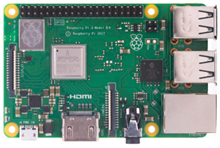
\includegraphics{Images/rpi3-modelB.png}
    \end{figure}



    \noindent \textcolor{red}{Example of table without caption:}
    %%% Use this link for easy way to generate tables with Latex
    %%% https://www.latex-tables.com/
    \begin{table}[h]
\centering
\begin{tblr}{
  width = \linewidth,
  colspec = {Q[148]Q[792]},
  cells = {t},
  hlines,
  vlines,
}
Processor           & {Broadcom
BCM2837B0, Cortex-A53\\64-bit SoC @ 1.4GHz~ ~~}                                                                                                                                                                                                                                                                              \\
GPU                 & Dual
Core VideoCore IV® Multimedia Co-Processor                                                                                                                                                                                                                                                                                        \\
Memory              & 1GB
LPDDR2 SDRAM                                                                                                                                                                                                                                                                                                                       \\
Connectivity        & {\labelitemi\hspace{\dimexpr\labelsep+0.5\tabcolsep}2.4GHz and 5GHz IEEE 802.11.b/g/n/ac wireless LAN, Bluetooth 4.2, BLE (Bluetooth Low Energy)\\\labelitemi\hspace{\dimexpr\labelsep+0.5\tabcolsep}Gigabit Ethernet over USB 2.0 (maximum throughput 300Mbps)\\\labelitemi\hspace{\dimexpr\labelsep+0.5\tabcolsep}4 × USB 2.0 ports} \\
{Video
and \\Sound} & {\labelitemi\hspace{\dimexpr\labelsep+0.5\tabcolsep}1 × full size HDMI\\\labelitemi\hspace{\dimexpr\labelsep+0.5\tabcolsep}MIPI DSI display port\\\labelitemi\hspace{\dimexpr\labelsep+0.5\tabcolsep}MIPI CSI camera port\\\labelitemi\hspace{\dimexpr\labelsep+0.5\tabcolsep}4 pole stereo output and composite video port}           \\
Multimedia          & H.264,
MPEG-4 decode (1080p30); H.264 encode
(1080p30); OpenGL ES 1.1, 2.0 graphics~ ~~                                                                                                                                                                                                                                               \\
SD Card Support     & Micro
SD format for loading operating system and data storage~ ~~                                                                                                                                                                                                                                                                      \\
Input Power         & {\labelitemi\hspace{\dimexpr\labelsep+0.5\tabcolsep}5V/2.5A DC via micro USB connector\\\labelitemi\hspace{\dimexpr\labelsep+0.5\tabcolsep}5V DC via GPIO header\\\labelitemi\hspace{\dimexpr\labelsep+0.5\tabcolsep}Power over Ethernet (PoE)–enabled (requires separate PoE HAT)}                                                    \\
Environment         & Operating
temperature, 0–50°C                                                                                                                                                                                                                                                                                                          \\
Dimensions          & 85 x
56 x 17mm                                                                                                                                                                                                                                                                                                                         
\end{tblr}
\end{table}


\clearpage{}
\newpage
\thispagestyle{empty}
\addtocontents{toc}{\string\contentsline{section}{\protect\hyperlink{appendixb}{APPENDIX - B}}{} \\}
\begin{center}
    {\bfseries \hypertarget{appendixb}{APPENDIX - B} }
    \vspace{1\baselineskip}
\end{center}

%%% PLACE BELOW YOUR APPENDIX %%%
\subsection*{Python Code Snippet} \addtocontents{toc}{\string\contentsline{subsection}{\protect\hyperlink{appendixb}{Python Code Snippet}}{} \\}

%% place actual code inside <lstlisting>
%% default is Python, to change use the command: \lstset{language=Java}
%% change the formatting in _preamble.tex

\begin{lstlisting}
# example for importing files or modules
import mymodule
from mypackage import mymodule
import mymodule as oMyFunction
from math import *

# example string
filePath = "/path/to/string.txt"

# example function
def incmatrix(genl1,genl2):
    m = len(genl1)
    n = len(genl2)
    M = None #to become the incidence matrix
    VT = np.zeros((n*m,1), int)  #dummy variable
    
    #compute the bitwise xor matrix
    M1 = bitxormatrix(genl1)
    M2 = np.triu(bitxormatrix(genl2),1) 

    for i in range(m-1):
        for j in range(i+1, m):
            [r,c] = np.where(M2 == M1[i,j])
            for k in range(len(r)):
                VT[(i)*n + r[k]] = 1;
                VT[(i)*n + c[k]] = 1;
                VT[(j)*n + r[k]] = 1;
                VT[(j)*n + c[k]] = 1;
                
                if M is None:
                    M = np.copy(VT)
                else:
                    M = np.concatenate((M, VT), 1)
                
                VT = np.zeros((n*m,1), int)
    
    return M
\end{lstlisting}


\clearpage{}

%%--- END OF PAPER
\end{document}
